% =========================================================================
% MÓDULO 2: DATOS, PIPELINE P0 Y AISLAMIENTO TEMPORAL (DIAPOSITIVAS 7 A 10)
% =========================================================================

% --- DIAPOSITIVA 7: COMPRENSIÓN DE DATOS Y BANDA HIGH-GAMMA ---
\begin{frame}{Comprensi\'on de Datos y Actividad Espectral High-Gamma}{Fundamento neurofisiol\'ogico de la banda $40\text{--}200\text{ Hz}$ para decodificaci\'on digital fina \cite{kaplan2019decoding,Bundy2016,gruenwald2023highgamma}}
  \begin{columns}[c,onlytextwidth]
    \begin{column}{0.39\textwidth}
      \begin{block}{Biomarcadores Corticales en ECoG}
        \scriptsize
        \begin{itemize}\setlength{\itemsep}{3.5pt}
          \item \textbf{Bandas $\mu / \beta$ ($8\text{--}30\text{ Hz}$):} Exhiben desincronizaci\'on (ERD) difusa y no espec\'ifica al inicio del movimiento.
          \item \textbf{Banda High-Gamma ($40\text{--}200\text{ Hz}$):} Refleja el disparo poblacional neuronal local en la capa V de la corteza motora primaria (M1) \cite{Bundy2016,gruenwald2023highgamma}.
          \item \textbf{Selectividad somatot\'opica:} La potencia High-Gamma se correlaciona de forma directa y focalizada con la cinem\'atica individual de cada dedo \cite{kaplan2019decoding}.
        \end{itemize}
      \end{block}
    \end{column}

    \begin{column}{0.58\textwidth}
      \centering
      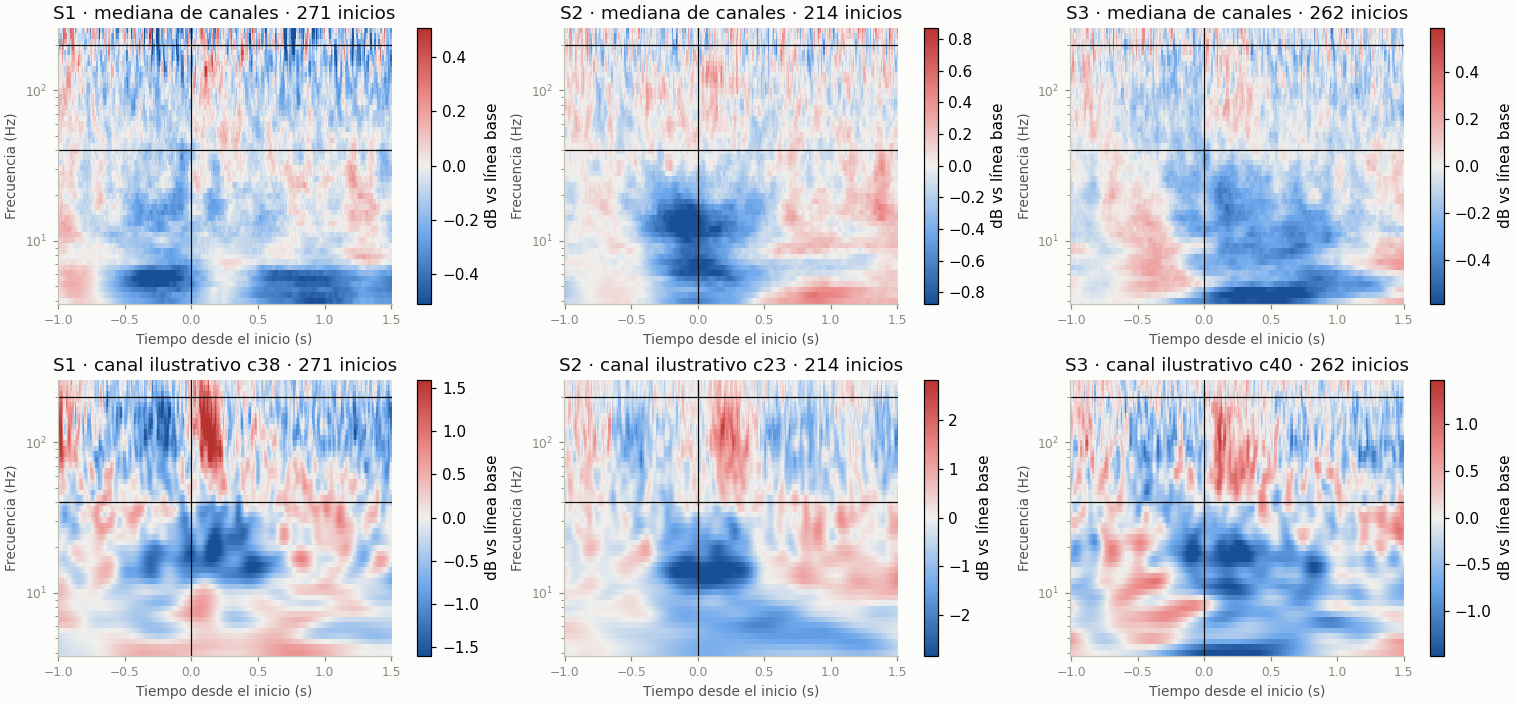
\includegraphics[width=\linewidth,height=0.54\textheight,keepaspectratio]{imgs/s04_ersp.png}
      \figcap{4}{Perturbaci\'on espectral ligada a eventos (ERSP) durante episodios de movimiento frente a reposo en la banda High-Gamma ($40\text{--}200\text{ Hz}$).}
    \end{column}
  \end{columns}

  \takeaway{La concentraci\'on de energ\'ia motora en la banda $40\text{--}200\text{ Hz}$ justifica el uso de un banco denso de \textbf{40 ond\'iculas complejas de Morlet} para capturar la envolvente instant\'anea de potencia en cada canal \cite{kaplan2019decoding,rodas_valencia_tpe_ecog}.}
\end{frame}

% --- DIAPOSITIVA 8: PIPELINE DE PROCESAMIENTO P0 ---
\begin{frame}{Pipeline de Procesamiento \texttt{P0}: Secuencia Matem\'atica}{Acondicionamiento tiempo-frecuencia reproducible de $1000\text{ Hz}$ a $100\text{ Hz}$ \cite{kaplan2019decoding,rodas_valencia_tpe_ecog}}
  % Diagrama de flujo horizontal limpio en TikZ
  \centering
  \begin{tikzpicture}[
    node distance=2.2mm,
    pbox/.style={rectangle, rounded corners=1.5mm, draw=ipnDark, fill=ipnSoft, thick, minimum height=9mm, inner sep=1.2mm, text width=1.82cm, align=center, font=\tiny\bfseries, text=textDark},
    arr/.style={-{Stealth[length=1.8mm]}, thick, ipnDark}
  ]
    \node[pbox] (b1) {1. Exclusi\'on y Clip\\$\pm 25\,\hat{\sigma}_{\text{MAD}}$};
    \node[pbox, right=of b1] (b2) {2. Referencia\\Mediana (CMR)};
    \node[pbox, right=of b2] (b3) {3. FIR Pasabanda\\y Notch Triple};
    \node[pbox, right=of b3] (b4) {4. CWT Morlet\\40 Bandas Log};
    \node[pbox, right=of b4] (b5) {5. Kaiser $100\text{ Hz}$\\Recorte $\pm 125$};
    \node[pbox, right=of b5, fill=rowHighlight] (b6) {6. Escalado Train\\Ventanas $W=256$};
    \draw[arr] (b1) -- (b2);
    \draw[arr] (b2) -- (b3);
    \draw[arr] (b3) -- (b4);
    \draw[arr] (b4) -- (b5);
    \draw[arr] (b5) -- (b6);
  \end{tikzpicture}

  \vspace{2mm}
  \begin{columns}[T,onlytextwidth]
    \begin{column}{0.48\textwidth}
      \begin{block}{Etapas 1 a 3: Limpieza y Filtrado Espectral}
        \scriptsize
        \begin{itemize}\setlength{\itemsep}{3pt}
          \item \textbf{Exclusi\'on fija + Clip MAD:} Canales v\'alidos ($\text{S1}:61, \text{S2}:46, \text{S3}:63$) y acotamiento $\pm 25\,\hat{\sigma}_{\text{MAD}}$.
          \item \textbf{Referencia Mediana Com\'un (CMR):} Sustracci\'on de la mediana espacial instant\'anea, inmune a valores at\'ipicos residuales.
          \item \textbf{Filtros FIR de fase cero:} Pasabanda en $\mathbf{40\text{--}200\text{ Hz}}$ ($331$ taps) y Notch en $\mathbf{60, 120, 180\text{ Hz}}$ ($1651$ taps).
        \end{itemize}
      \end{block}
    \end{column}

    \begin{column}{0.48\textwidth}
      \begin{block}{Etapas 4 a 6: Escalograma, Decimaci\'on y Escalado}
        \scriptsize
        \begin{itemize}\setlength{\itemsep}{3pt}
          \item \textbf{40 Wavelets de Morlet ($n_c=7$):} Potencia instant\'anea $P_{c,f_i}(t) = |(x_c * \psi_{f_i})(t)|^2$ en escala logar\'itmica.
          \item \textbf{Decimaci\'on Kaiser a $100\text{ Hz}$:} Filtro FIR antialias ($243$ taps) y eliminaci\'on de $\mathbf{\pm 125\text{ muestras}}$ de borde ($1250\text{ ms}$).
          \item \textbf{Escalado sin fuga:} \texttt{RobustScaler}$(10,90)$ en ECoG y \texttt{MinMaxScaler}$[0,1]$ en guante, ajustados \textbf{solo en train}.
        \end{itemize}
      \end{block}
    \end{column}
  \end{columns}
\end{frame}

% --- DIAPOSITIVA 9: RECONSTRUCCIÓN CINEMÁTICA DEL GUANTE Y ADELANTO FISIOLÓGICO ---
\begin{frame}{Reconstrucci\'on Cinem\'atica del Guante y Adelanto Fisiol\'ogico}{Recuperaci\'on de muestras efectivas ZOH ($25\text{ Hz}$) e interpolaci\'on por Spline C\'ubico a $100\text{ Hz}$ \cite{miller2008prediction,rodas_valencia_tpe_ecog}}
  \begin{columns}[c,onlytextwidth]
    \begin{column}{0.39\textwidth}
      \begin{block}{Acondicionamiento de Etiquetas $y_d(t)$}
        \scriptsize
        \begin{itemize}\setlength{\itemsep}{3.5pt}
          \item \textbf{Problema del ZOH crudo:} El guante actualiza su lectura cada $40\text{ ms}$ ($25\text{ Hz}$), generando escalones artificiales con derivadas nulas y saltos discontinuos.
          \item \textbf{Interpolaci\'on Spline C\'ubico (\textit{Not-a-Knot}):} Se extraen los nodos reales ($n=40m$) y se reconstruye una curva suave con continuidad $C^2$ a $\mathbf{100\text{ Hz}}$.
          \item \textbf{Adelanto fisiol\'ogico ($\mathbf{\tau = 20\text{ ms}}$):} Desplazamiento de $+2\text{ muestras}$ a $100\text{ Hz}$ para alinear el comando motor cortical con la ejecuci\'on mec\'anica perif\'erica.
        \end{itemize}
      \end{block}
    \end{column}

    \begin{column}{0.58\textwidth}
      \centering
      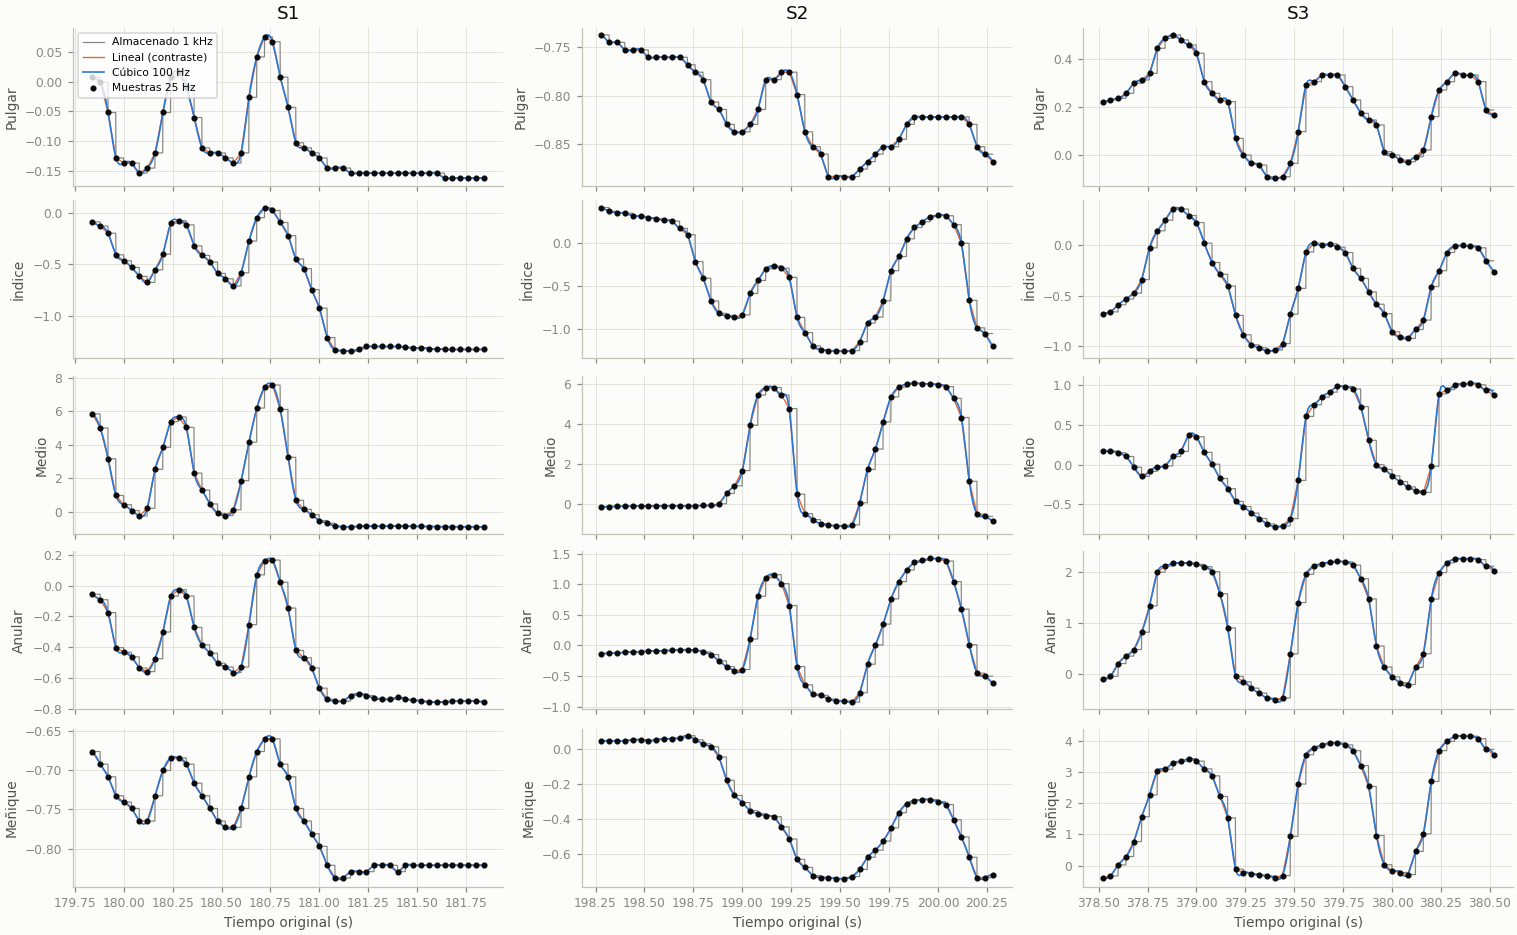
\includegraphics[width=\linewidth,height=0.48\textheight,keepaspectratio]{imgs/s08_glove_interpolation.png}
      \figcap{5}{Comparaci\'on entre la se\~nal escalonada original del guante (ZOH a $25\text{ Hz}$) y la trayectoria continua reconstruida mediante Spline C\'ubico a $100\text{ Hz}$.}
    \end{column}
  \end{columns}

  \takeaway{La interpolaci\'on por Spline C\'ubico elimina los artefactos de escal\'on del dataglove y permite entrenar la red neuronal con objetivos cinem\'aticos f\'isicamente diferenciables \cite{rodas_valencia_tpe_ecog}.}
\end{frame}

% --- DIAPOSITIVA 10: AISLAMIENTO TEMPORAL Y VALIDACIÓN POR BLOQUES ---
\begin{frame}{Aislamiento Temporal y Validaci\'on sin Fuga de Informaci\'on}{Esquema de validaci\'on cruzada en $K=5$ bloques cronol\'ogicos con zona de purga $P=256$ \cite{roberts2017crossvalidation,rodas_valencia_tpe_ecog}}
  \begin{columns}[c,onlytextwidth]
    \begin{column}{0.39\textwidth}
      \begin{block}{Blindaje contra \textit{Data Leakage}}
        \scriptsize
        \begin{itemize}\setlength{\itemsep}{2.5pt}
          \item \textbf{Partici\'on en $K=5$ bloques (\texttt{B1--B5}):} Cada bloque de $80\text{ s}$ se procesa de forma independiente (aislamiento de filtros FIR y wavelets).
          \item \textbf{Recorte de soporte DSP ($\mathbf{\pm 125}$):} Se descartan los extremos transitorios ($165+825+139+121=1250$ muestras a $1\text{ kHz}$), dejando $N=7750$ muestras v\'alidas por bloque.
          \item \textbf{Margen de purga ($\mathbf{P = 256}$):} Con ventanas deslizantes de $W=256$ ($2.56\text{ s}$), se aplica una purga de $256\text{ muestras}$ para garantizar solapamiento $\mathbf{0.0}$ entre train y val \cite{roberts2017crossvalidation}.
        \end{itemize}
      \end{block}
    \end{column}

    \begin{column}{0.58\textwidth}
      \centering
      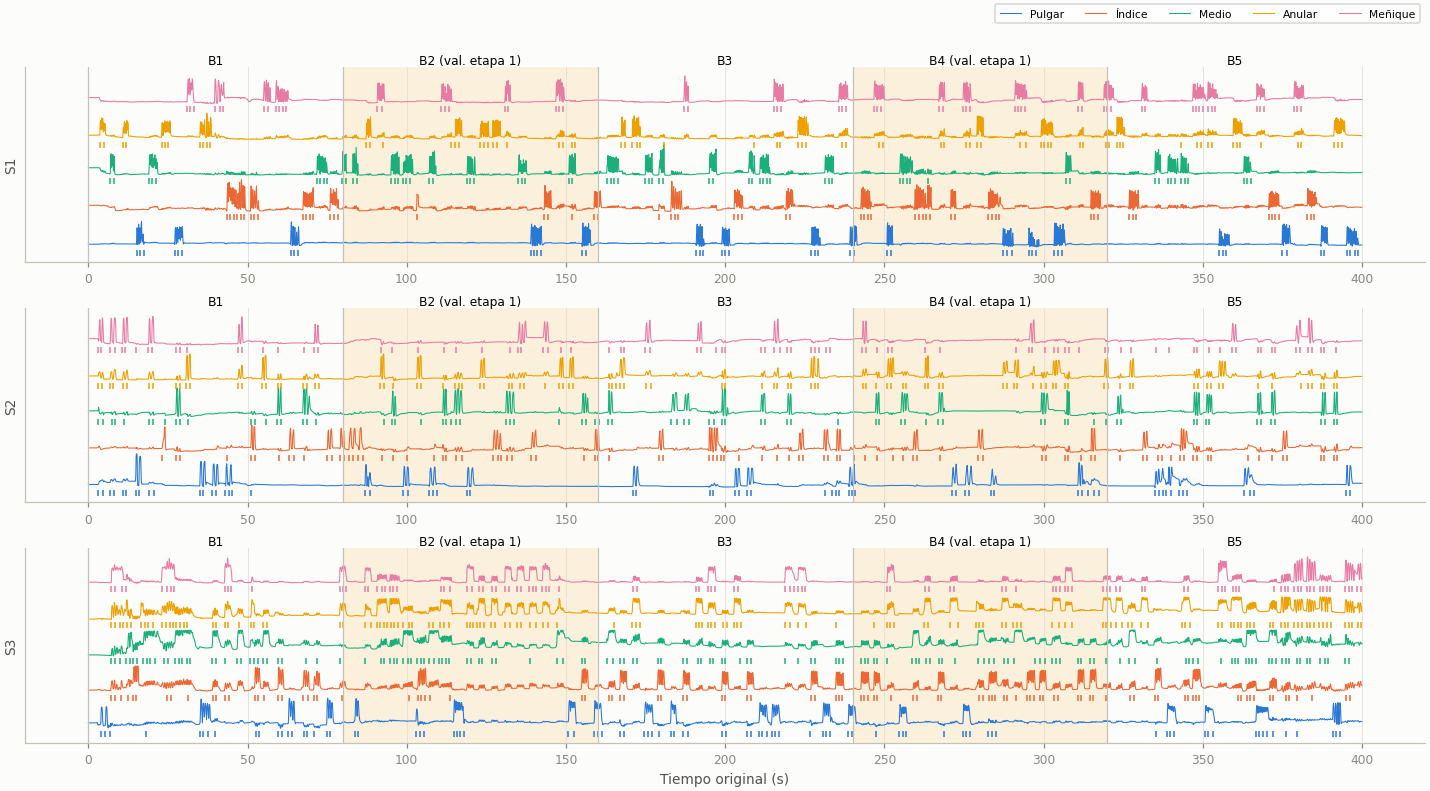
\includegraphics[width=\linewidth,height=0.46\textheight,keepaspectratio]{imgs/s11_blocks_timeline.png}
      \figcap{6}{Estructura de los 5 bloques cronol\'ogicos (\texttt{B1--B5}), recorte de bordes transitorios ($\pm 125$) y zona de purga ($P=256$ muestras) verificada por las compuertas \texttt{V01--V14}.}
    \end{column}
  \end{columns}

  \takeaway{A diferencia de una partici\'on aleatoria de ventanas (que infla artificialmente Pearson por autocorrelaci\'on temporal), la validaci\'on por bloques purgados eval\'ua la generalizaci\'on real en segmentos futuros no vistos \cite{roberts2017crossvalidation}.}
\end{frame}
